% ===========================================================================
% SECTION 2 — SYSTEM MODELING
% Target: 600-800 words
% ===========================================================================

\section{System Modeling}
\label{sec:system_modeling}

\subsection{NREL 5-MW Reference Turbine}
\label{subsec:nrel5mw}

This study uses the NREL offshore 5-MW reference wind turbine
\citep{jonkman2009} as the physical plant. This model is widely adopted as a
benchmark in the wind energy control literature, which allows direct
comparison with previously published MPC and ML-surrogate studies. The
turbine has a rotor radius $R = \SI{63}{m}$, a combined drivetrain inertia
$J = 3.876 \times 10^{7}~\text{kg}\cdot\text{m}^2$ (referred to the
low-speed shaft, LSS), a $97{:}1$ gearbox ratio, a rated rotor speed
$\omegarated = \SI{12.1}{rpm}$, and a rated generator torque (high-speed
shaft, HSS) $T_{g,\text{rated}} = P_{\text{rated}} / (\omegarated
N_{\text{gear}}) = \SI{40680}{N.m}$. The rated tip-speed ratio is
$\lambda_{\text{rated}} = 7.00$. Full turbine parameters are reported in
Table~\ref{tab:turbine_params}.

\begin{table}[H]
\centering
\caption{NREL 5-MW reference turbine parameters used in this study
(source: \citet{jonkman2009}, with the drivetrain damping and torque
switching calibration choices documented in Section~\ref{subsec:torque_switching}).}
\label{tab:turbine_params}
\begin{tabular}{lcc}
\toprule
Parameter & Symbol & Value \\
\midrule
Rotor radius              & $R$                 & \SI{63}{m} \\
Number of blades          & $B$                 & 3 \\
Air density                & $\rho$              & \SI{1.225}{kg/m^3} \\
Drivetrain inertia (LSS)   & $J$                 & $3.876\times10^{7}$ kg$\cdot$m$^2$ \\
Drivetrain damping         & $B_r$               & \SI{6215.5}{N.m.s/rad} \\
Gear ratio                 & $N_{\text{gear}}$   & 97 \\
Pitch actuator time constant & $\tau_\beta$      & \SI{0.1}{s} \\
Pitch bounds                & $\beta$             & $[0,\ 25]\deg$ \\
Maximum pitch rate          & $\dot\beta_{\max}$  & \SI{8.0}{deg/s} \\
Rated rotor speed          & $\omegarated$       & \SI{12.1}{rpm} \\
Physical min.\ rotor speed & $\omega_{\min}$     & \SI{4.77}{rpm} \\
Overspeed limit (+10\%)    & $\omega_{\max}$     & \SI{13.31}{rpm} \\
Rated tip-speed ratio       & $\lambda_{\text{rated}}$ & 7.00 \\
Rated power                & $P_{\text{rated}}$  & \SI{5}{MW} \\
Rated wind speed           & $V_{\text{rated}}$  & \SI{11.4}{m/s} \\
Cut-in wind speed          & $V_{\text{in}}$     & \SI{3.0}{m/s} \\
Cut-out wind speed         & $V_{\text{out}}$    & \SI{25.0}{m/s} \\
Rated generator torque (HSS) & $T_{g,\text{rated}}$ & \SI{40680}{N.m} \\
Region II gain (LSS)        & $\Kopt$             & $2.5106\times10^{6}$~N.m.s$^2$ \\
\bottomrule
\end{tabular}
\end{table}

\subsection{Two-State Model}
\label{subsec:two_state_model}

Following the modeling approach of \citet{klein2024}, the turbine is
represented by a reduced two-state nonlinear model with state vector
$x = [\omegar, \beta]^\top$, control input $u = \betacmd$ (pitch angle
demand), and measured disturbance $V$ (rotor-effective wind speed). The
rotor dynamics are governed by the aerodynamic torque balance

\begin{equation}
J\,\dot{\omegar} = \Ta(\omegar, \beta, V) - \Tg^{\text{LSS}}(\omegar) - B_r\,\omegar,
\label{eq:rotor_ode}
\end{equation}

where $\Tg^{\text{LSS}}$ is the generator reaction torque referred to the
low-speed shaft (Section~\ref{subsec:torque_switching}), $B_r =
\SI{6215.5}{N.m.s/rad}$ is a linear drivetrain damping coefficient
(Table~\ref{tab:turbine_params}), and the
aerodynamic torque is
$\Ta = \tfrac{1}{2}\rho \pi R^2 V^3 \Cp(\lambda,\beta) / \omegar$, with tip-speed
ratio $\lambda = \omegar R / V$ and power coefficient surface
$\Cp(\lambda,\beta)$ evaluated with the Jonkman polynomial. The pitch
actuator is modeled as a first-order lag,

\begin{equation}
\tau_\beta\,\dot{\beta} = \betacmd - \beta,
\label{eq:pitch_actuator}
\end{equation}

with $\tau_\beta = \SI{0.1}{s}$. Equations~\eqref{eq:rotor_ode}--\eqref{eq:pitch_actuator}
are integrated with explicit Euler discretization at $\Delta t = \SI{0.1}{s}$,
matching the control sampling time $T_s$ used by the nonlinear MPC in
Section~\ref{sec:mpc_framework}. The $\Cp(\lambda,\beta)$ surface is
evaluated strictly within its calibration domain $\beta \in [0\deg, 25\deg]$;
Stage~0 validation confirmed a maximum power coefficient
$\Cp^{\max} = 0.480$ at $\lambda^{*} = 8.11$, $\beta^{*} = 0\deg$, safely
below the Betz limit ($C_{p,\text{Betz}} = 0.5926$), correcting an earlier
non-physical evaluation of the polynomial outside its calibrated range that
had produced $\Cp^{\max} = 0.706 > C_{p,\text{Betz}}$.

\subsection{Region II/III Generator Torque Switching}
\label{subsec:torque_switching}

A methodological contribution of this work concerns the generator torque
model $\Tg^{\text{LSS}}(\omegar)$ in Eq.~\eqref{eq:rotor_ode}. An initial
implementation assumed a constant rated torque
$\Tg^{\text{LSS}} = N_{\text{gear}}\,T_{g,\text{rated}}$ at all rotor
speeds. Under this assumption, long-horizon closed-loop simulation revealed
an irrecoverable operating trap: for $\omegar$ below the rated speed, the
aerodynamic torque $\Ta$ available at low wind speed can fall below the
constant demanded generator reaction torque, driving $\dot{\omegar} < 0$
with no control authority left to arrest the deceleration (the pitch angle
is already saturated at its lower bound $\beta = 0\deg$), so the rotor
stalls toward zero speed.

This was corrected by replacing the constant-torque assumption with the
standard Region~II/III generator torque switching law, expressed
consistently in low-speed-shaft (LSS) torque on both sides,

\begin{equation}
\Tg^{\text{LSS}}(\omegar) =
\begin{cases}
\Kopt\,\omegar^{2}, & \omegar < \omegarated \quad \text{(Region II)} \\[4pt]
N_{\text{gear}}\,T_{g,\text{rated}}, & \omegar \geq \omegarated \quad \text{(Region III)}
\end{cases}
\label{eq:torque_switching}
\end{equation}

where $\Kopt = \tfrac{1}{2}\rho A_{\text{rotor}} \Cp(\lambda_{\text{rated}})
R^3 / \lambda_{\text{rated}}^3 = 2.5106\times10^{6}~\text{N.m.s}^2$ is
calibrated at the actual Jonkman operating point
$\lambda_{\text{rated}} = R\,\omegarated / V_{\text{rated}} = 7.00$, rather
than the theoretical aerodynamic optimum $\lambda^{*} = 8.11$ identified in
Section~\ref{subsec:two_state_model}. This choice follows standard practice
\citep[e.g.][]{jonkman2009}: Jonkman's rated operating point already
accounts for drivetrain and electrical losses, so it sits slightly off the
pure-aerodynamic $\Cp$ peak; calibrating $\Kopt$ there prioritizes torque
continuity at the switching boundary over exact aerodynamic optimality
(calibrating instead at $\lambda^{*}=8.11$ would produce a $30\%$
discontinuity, versus $2.26\%$ at $\lambda_{\text{rated}}=7.00$). The
resulting continuity ratio is
$\Kopt \omegarated^{2} / (N_{\text{gear}} T_{g,\text{rated}}) = 1.0226$,
i.e.\ a $2.26\%$ torque discontinuity at $\omegar = \omegarated$
(a single-point deficit of \SI{89108}{N.m} on the low-speed shaft,
$K_{\text{opt}}\omegarated^2 - N_{\text{gear}}T_{g,\text{rated}} =
\SI{4035098}{N.m} - \SI{3945990}{N.m}$), which is documented and accepted as
negligible: the explicit-Euler integration together with continuous
turbulent-wind excursions means the simulated system never dwells exactly
at $\omegar = \omegarated$ to machine precision. Feasibility of
Eq.~\eqref{eq:torque_switching} was validated by confirming
$\Ta(\omegar,\beta,V) - \Tg^{\text{LSS}}(\omegar) > 0$ for all
$\omegar \in [\omega_{\min}, \omegarated]$ and all $V$ in the operating
envelope, eliminating the trap. Fig.~\ref{fig:torque_switching} illustrates
$\Ta$ and $\Tg^{\text{LSS}}(\omegar)$ before and after the correction. This
correction also constrains the admissible rotor-speed range used for
surrogate-based MPC bounds in Stage~3
(Section~\ref{sec:mpc_framework}): the training domain identified in
Stage~1 (Section~\ref{sec:dataset_generation}) is $[8.02,13.31]$~rpm,
yielding surrogate MPC bounds of $[8.52,12.81]$~rpm with a
$\SI{0.5}{rpm}$ safety margin on each side, distinct from the wider
$[11.5,13.31]$~rpm defense-in-depth bound retained for the physics-based
Baseline controller.

\begin{figure}[H]
\centering
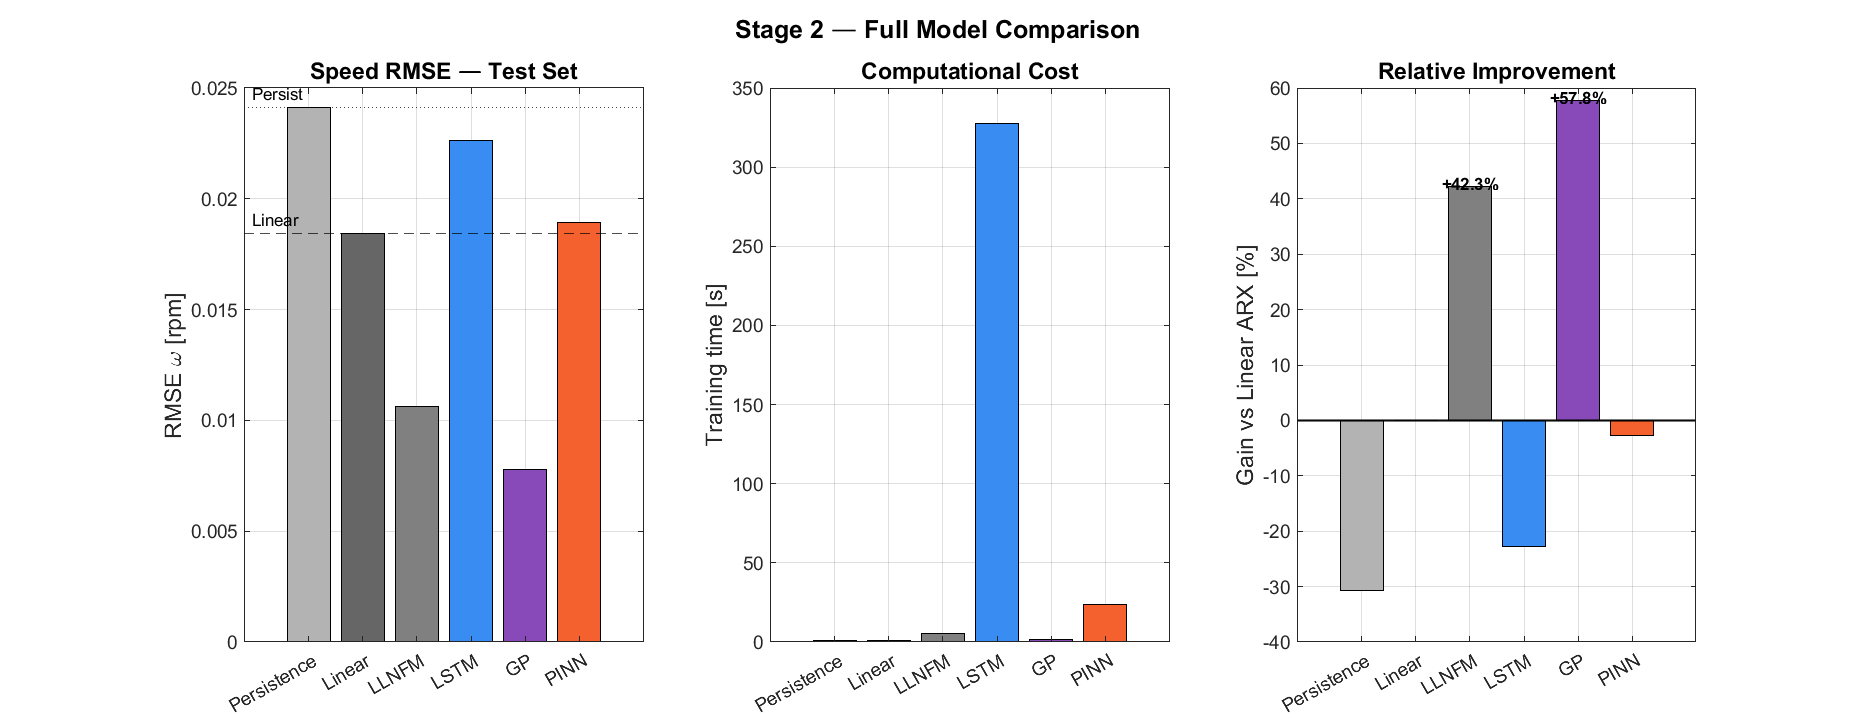
\includegraphics[width=0.8\textwidth]{figures/Fig3_S2_ModelSummary.png}
\caption{Region II/III generator torque switching: aerodynamic torque
$\Ta$ and generator torque $\Tg(\omegar)$ before (constant torque) and
after (Eq.~\eqref{eq:torque_switching}) correction.}
\label{fig:torque_switching}
\end{figure}

\subsection{Wind Model}
\label{subsec:wind_model}

Turbulent wind input is generated from the Kaimal spectrum defined in
IEC~61400-1 \citep{iec61400} with turbulence intensity $I = 0.16$,
longitudinal turbulence length scale $L_1 = \SI{340.2}{m}$. We note that
$I=0.16$ corresponds to IEC Turbulence Category~A (the more severe of
the two standard categories at this hub height) rather than
Category~B ($I=0.14$) as an earlier draft of this work mislabeled it;
the simulated turbulence is therefore somewhat more severe than a
Category-B label would imply, not less. Time series are
synthesized via inverse FFT of the discretized Kaimal power spectral
density, with the amplitude spectrum deterministically rescaled before
phase randomization so that the achieved standard deviation
$\sigma_{\text{actual}}$ matches the target
$\sigma_{\text{target}} = I \cdot V_{\text{mean}}$ \emph{by construction}
 this rescaling step is a normalization procedure, not an
independent validation of the synthesized turbulence, and should not
be read as evidence that the resulting time series matches the target
Kaimal spectrum in any property other than its overall standard
deviation; validating the achieved power spectral density shape
against the analytical Kaimal spectrum independently is noted as
future work. The
synthesized wind signal is subsequently passed through a second-order
Butterworth low-pass filter with cutoff frequency $f_c = \SI{0.3}{Hz}$,
consistent with the rotor-effective wind filtering approach of
\citet{klein2024}, before being applied as the disturbance input $V$ to
Eq.~\eqref{eq:rotor_ode}.
